\label{sec:sym_verschl}

Die symmetrische Verschlüsselung folgt dem Konzept, das sowohl für die Ver- als auch die Entschlüsselung jeweils die gleichen Schlüssel verwendet werden.

\begin{figure}[h!]
	\centering
	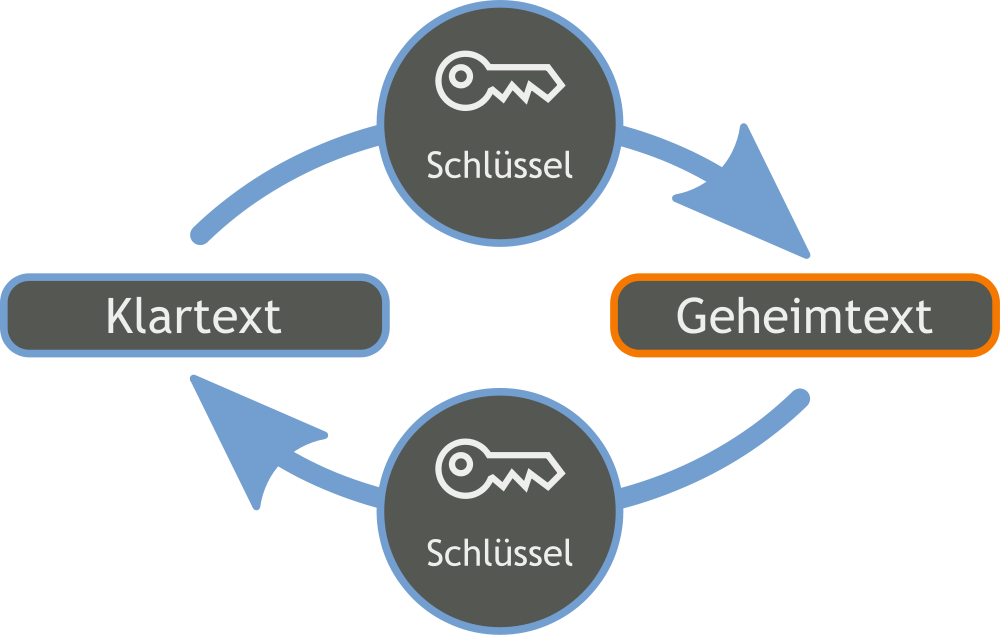
\includegraphics[width=\linewidth]{img/SymKrypto.png}
	\caption{Symmetrische Verschlüsselung mit identischen Schlüsseln}
	\label{fig:sym_verschl}
	\end{figure}
	\footnotetext{Quelle: Bananenfalter (Public Domain) \\ \url{https://commons.wikimedia.org/wiki/File:Orange_blue_symmetric_cryptography_de.svg}}

Es gibt eine Reihe an unterschiedlichsten Algorithmen und Verfahren für symmetrische Verschlüsselung, allerdings hat sich mit \textsc{AES} ein Verfahren als de-facto Standard für verschiedenste Anwendungsbereiche etabliert.

AES ist hierbei eine Abkürzung für Advanced Encryption Standard und wird meist synonym für den Rijndael-Algorithmus verwendet. Dieses Verfahren ist heute so verbreitet, dass beispielsweise in modernen Prozessoren direkt als Maschinenbefehl zur Verfügung steht und somit deutlich größere Datenraten verarbeiten kann. \\
Benchmarks zeigen hier beispielshaft einen 6-fachen Speedup mit einer Datenrate von ca. 1.35 GB/s mit CPU-Unterstützung verglichen mit 212 MB/s ohne
CPU-Unterstützung.\footnote{aes:benchmark}

Vor allem durch die Hardware-Unterstützung ist es moderner Ransomware möglich, die CPU-Last während der Verschlüsselung derart in Grenzen zu halten, dass der Nutzer keine spürbare Langsamkeit des Systems bemerkt.


\subsection{Asymmetrische Verschlüsselung}
\label{sec:asym_verschl}

\begin{figure}[h!]
	\centering
	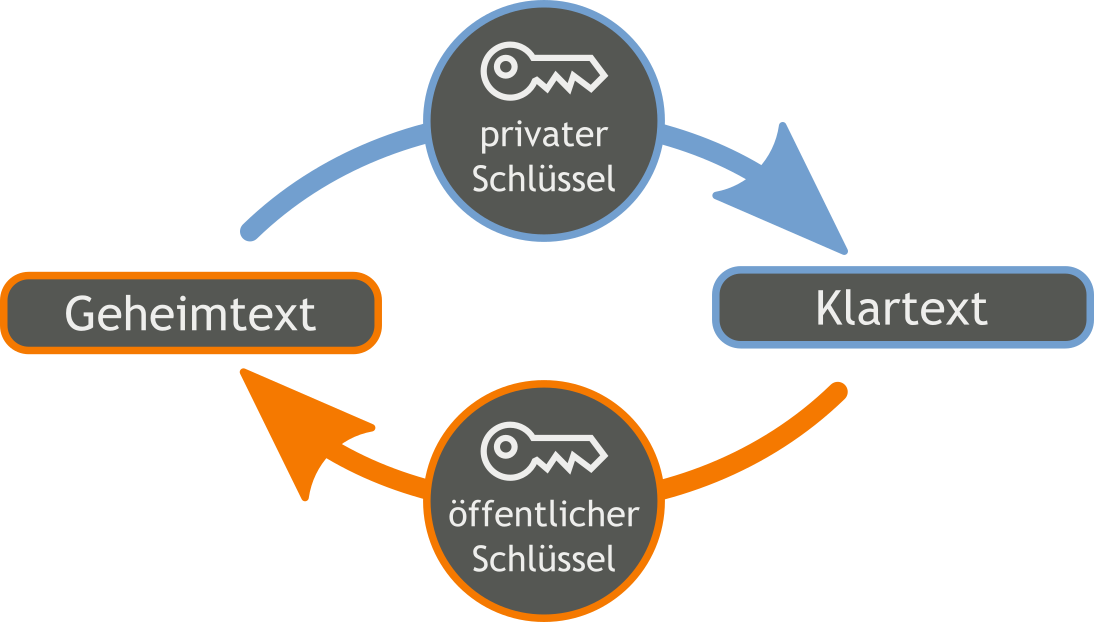
\includegraphics[width=\linewidth]{img/AsymKrypto.png}
	\caption{Asymmetrische Verschlüsselung}
	\label{fig:asym_verschl}
	\end{figure}
	\footnotetext{Quelle: Bananenfalter (Public Domain) \\ \url{https://commons.wikimedia.org/wiki/File:Orange_blue_symmetric_cryptography_de.svg}} %TODO: Url


Asymmetrische Verschlüsselung basiert auf zwei Schlüsseln, einen öffentlichen und einen privaten. Diese Schlüssel gehören mathematisch zusammen und werden für unterschiedliche Zwecke verwendet.
Soll ein Klartext verschlüsselt werden, so wird hierfür der öffentliche Schlüssel des Empfängers verwendet. Die Entschlüsselung muss dann mit dem zugehörigen privaten Schlüssel erfolgen, eine Entschlüsselung mit dem öffentlichen Schlüssel ist nicht mehr möglich.

Auf Grund der Komplexität der Berechnungen ist das Verfahren langsam und auch nur schwer in Hardware abzubilden. Deshalb wird es nur für verhältnismäßig kurze Klartexte verwendet (< 1 KB), auch da die maximale Länge des Klartexts von der Länge des verwendeten Schlüssels abhängt. %TODO: Nachweis


Der große Vorteil von asymmetrischer Verschlüsselung liegt im sicheren Schlüsselaustausch, der nicht auf einen bereits gesicherten Kanal angewiesen ist, sondern auch über ein unsicheres Medium, beispielsweise über das Internet erfolgen kann, ohne dass es für einen Angreifer möglich ist die beteiligten Schlüssel zu belauschen oder zu berechnen. %TODO: MitM




\subsection{Hybride Verschlüsselung}
\label{sec:hybride_verschl}

Hybride Verschlüsselung kombiniert alle Vorteile von symmetrischer Verschlüsselung (Geschwindigkeit, Einfachheit) mit allen Vorteilen von asymmetrischer Verschlüsselung (Schlüsseltausch, Sicherheit).
Hierfür werden zufällige Schlüssel erzeugt, meist lange Zufallszahlen, die für die symmetrische Verschlüsselung verwendet werden. Diese Schlüssel werden Sitzungsschlüssel genannt und werden in der Regel nur einmalig verwendet (ein sog. One-Time-Pad). Nach der Verwendung werden die Sitzungsschlüssel asymmetrisch verschlüsselt und mit den codierten Daten zusammen übertragen.

Auf diese Weise lassen sich auch große Mengen an Daten effizient mittels asymmetrischer Kryptographie übertragen.
